\section{Interfejs MPI}

\subsection{Model sieciowy}

Komunikacja odbywa sie za pomocą przesyłania wiadomości (czyli między innymi w standardzie MPI)w tak zwanym modelu sieciowym. Składa się on z określonej liczby procesorów, przy czym każdy z nich posiada własną pamięć lokalną. Procesory posiadają dostęp jedynie do instrukcji i danych przechowywanych w swojej pamięci lokalnej -- nie istnieje pamięć wspólna. Aby umożliwić wymianę informacji pomiędzy procesorami, tworzona jest sieć połączeń (ang \textit{interconnection network}), która zbudowana jest z dwukierunkowych kanałów komunikacyjnych (łącz). 

\begin{figure}[h]
	\centering
	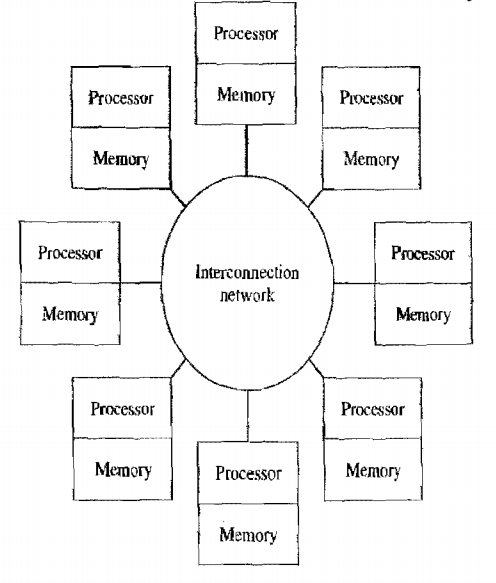
\includegraphics[width=0.85\textwidth]{./img/sieciowy.png}
	\caption{Model sieciowy. Źródło: \cite{Parallel}, str 94}
	\label{img:sieć}
\end{figure}

Wymiana informacji między procesorami jest realizowana poprzez kooperujące ze sobą procedury trasowania (ang. \textit{routing}), które działają w każdym procesorze. Dzięki nim, każdy węzeł sieci (tutaj: procesor) posiada informację, z którymi węzłami może wymieniać informacje. Zbiór wszystkich procedur trasowania definiuje \textbf{topologię sieci połączeń}. Można ją opisać przy pomocy grafu, gdzie wierzchołkami (węzłami) są procedory, natomiast krawędzi to dwukierunkowe łącza.

Ocenę skuteczność/przydatność danej sieci podczas prowadzenia obliczeń równoległych można określić biorąc pod uwagę kilka parametrów:

\begin{itemize}
	\item \textbf{Średnica sieci} (ang \textit{diameter}) -- maksymalna odległość zmierzoną za pomocą liczby krawędzi między dowolnymi dwoma wierzchołkami. Im mniejsza średnica, tym lepsza jest sieć -- oznacza to, że informacje będą potrzebowały średnio mniej czasu na dotarcie do właściwego odbiorcy. Przypadek pesymistyczny zakłada, że wiadomość będzie musiała zostać przesłana przez liczbę krawędzi równej średnicy.
	\item \textbf{Szerokość połowienia sieci} (ang. \textit{bisection width}) -- minimalna liczba krawędzi, którą należy usunąć z obecnej sieci, aby móc ją podzielić na 2 równe podsieci.
	\item \textbf{Szerokość pasma} (ang. \textit{bisection bandwidth}) -- jest to iloczyn szerokości połowienia oraz szybkości przesyłu danych w pojedynczym kanale. Pozwala określić liczbę bitów, jaką można przesłać między połówkami w jednostce czasu. Im większa szerokość pasma, tym lepiej.
	\item \textbf{Maksymalny stopień wierzchołka} -- maksymalna liczba krawędzi połączonych z danym wierzchołkiem (liczona globalnie dla całej sieci). Dla niewielkiego stopnia łatwiej zaprogramować procedury komunikacyjne ze względu na fakt, że używają one mniejszej liczby kanałów. Zakłada się, że sieć jest dobra jeżeli przy wzroście liczby p procesorów średnica sieci rośnie nie szybciej niż logarytmicznie w funkcji p, natomiast maksymalny stopień wierzchołka jest stałą liczbą o małej wartości.
	\item \textbf{Spójność krawędziowa} (ang. \textit{edge connectivity}) -- definiowana jaka minimalna liczba krawędzi, które muszą zostać wyłączone z sieci aby ta stała się niespójna (graf rozłoży się na 2 lub więcej osobnych podgrafów). Im większa spójność krawędziowa, tym odporniejsza jest sieć -- istnieje mniejsze prawdopodobieństwo całkowitego unieruchomienia sieci w przypadku, gdy któryś procesor ulegnie uszkodzeniu. Większa spójność prowadzi też do zmniejszenia rywalizacji poszczególnych węzłów o łącze.
	\item \textbf{Koszt sieci} -- zazwyczaj określana jako suma wszystkich kanałów w sieci.
\end{itemize}

Przykładowe topologie sieci połączeń:

\begin{itemize}
	\item siatka
	\item torus (jedno-, wielowymiarowy)
	\item kostka (jedno-, wielowymiarowa)
\end{itemize}

\begin{figure}[h]
	\centering
	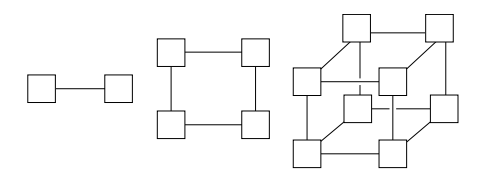
\includegraphics[width=0.85\textwidth]{./img/kostki.png}
	\caption{Topologia kostki. Od lewej: jedno-, dwu- oraz trójwymiarowa. Źródło: \cite{Pacheco}, str 40}
	\label{img:sieć}
\end{figure}

\subsection{Zasada działania MPI}

MPI jako interfejs przeznaczony do pracy z obliczeniami rozproszonymi oparty został o model sieciowy, posiadaja jednak kilka cech, które wyróżniają od standardowej implementacji tego wzorca. MPI można potraktować jako interfejs pomiędzy programem a systemem operacyjnym.

Tradycyjnie, każdy z procesów posiada własną pamięć lokalną, co narzuca konieczność komunikacji przez dwukierunkowe łącza kounikacyjne (w nomenklaturze MPI nazwywane \textbf{komunikatorami}). Komunikacja polega na przesłaniu danych z pamięci procesu źródłowego do pamięci lokalnej procesu docelowego przy wykorzystaniu węzłów pośrednich. Domyślnie każdy nowoutworzony proces znajduje się w komunikatorze świat (MPI\textunderscore COMM\textunderscore WORLD). Takie rozwiązanie sprawia, że każdy proces może wymieniać dane z dowolnym pośród pozostałych, niezależnie od fizycznej struktury procesorów (jest ona przezroczysta dla procesów). Istnieje możliwość zdefiniowania własnych komunikatorów -- co może okazać się przydatne w przypadku, gdy programista chce zawężyć zakres procesów, do których wysyłana jest wiadomość rozgłoszeniowa (ang. \textit{broadcast}).

W trakcie tworzenia programu w oparciu o ten interfejs, warto podzielić część programu przeznaczoną do obliczeń rozproszonych na części, które mają zostać przydzielone do osobnych procesów. Na początku pracy, deklarowana jest ilość procesów, które mają zostać zaangażowane do pracy. Może się to odbywać na jeden z 2 sposobów:

\begin{itemize}
	\item Statyczny -- procesy tworzone są przed wykonaniem programu. Program (proces główny, tak zwany \textit{root}) nie może zostać zakończony przed końcem pracy wszystkich pozostałych procesów.
	\item Dynamiczny -- Potrzebne procesy są tworzone podczas pracy programu. Ta opcja jest dostępna wyłącznie dla wersji MPI-2 (zaprezentowanej w 1997 roku).
\end{itemize}

Każdy utworzony proces posiada własny unikalny identyfikator (id) w ramach komunikatora. W różnych komunikatorach ten sam proces może posiadać różne id. Identyfikatorem procesu głównego (\textit{roota}) jest liczba 0.

W momencie tworzenia nowego procesu, tworzona jest kopia programu przeznaczonego tylko dla tego procesu. W praktyce oznacza to, że posiada dostęp do każdej zmiennej zadeklarowanej globalnie, jednak tylko w ramach lokalnej kopii. W przypadku, gdy proces potrzebuje danych znajdujących się w innym węźle, konieczna jest wymiana informacji w ramach komunikatora. Do rozdzielania pracy stosuje się standardowe operacje rozgałęzienia (między innymi instrukcje \textit{if} czy \textit{else} w językach C/C++) identyfikując id procesu. Jest to technika zwana SPMD (\textit{Single Program Multiple Data} -- pojedynczy program, wiele danych), będący subkategorią MIMD (\textit{Multiple Instruction Multiple Data} - wiele instrukcji, wiele danych), znanej z taksonomii Flynna. Zazwyczaj utworzone kopie programów działają w sposób asynchroniczny, lecz może dojść do sytuacji, w której procesy te będą działały synchronicznie. Określony sposób działania może być uzależniony od funkcji, jakie zostaną użyte przez programistę.

\subsection{Kompilacja i uruchamianie}

Szczegóły związane z kompilacją i uruchamianiem programu napisanego przy użyciu biblioteki MPI są zależne od używanego systemu operacyjnego. Większość z nich do kompilacji używa komendy, której można użyć z poziomu linii poleceń/terminala: \\

\texttt{\$ mpicc -g -Wall -o <plik\textunderscore źródłowy> <plik\textunderscore wynikowy>.c} \\

Zazwyczaj \texttt{mpicc} jest skryptem opakowującym (ang. \textit{wrapper script}) dla kompilatora języka (dla powyższego przypadku, języka C). Skrypt opakowujący jest pisany w celu uruchomienia określonego programu. Skrypt ten upraszcza uruchomienie kompilatora poprzez jawne wskazanie, w którym miejscu znajdują się potrzebne pliki nagłówkowe oraz które biblioteki nalezy połączyć z plikiem obiektu.

Uruchamianie skompilowanego programu odbywa się przez następującą komendę: \\

\texttt{mpirun -np <liczba\textunderscore procesów> <nazwa\textunderscore pliku\textunderscore wynikowego> <parametry>} \\

W wyżej wymienionej komendzie <liczba\textunderscore procesów> jest liczbą całkowitą dodatnią i wskazuje, ile procesów ma być wykonanych równolegle. <nazwa\textunderscore pliku\textunderscore wynikowego> oraz <parametry> przekazywane są do procesów za pośrednicztwem zmiennych \texttt{argc} i \texttt{argv} znajdujących się w nagłówku funkcji main (zgodnie z zasadami języka C).


\subsection{Inicjalizacja i kończenie programu}

Większość elementów składowych programu napisanego przy użyciu MPI jest instrukcjami natywnymi używanego języka (C, C++, Ada, Fortran). Aby umożliwić korzystanie z instrukcji nowej biblioteki, należy dodać następującą instrukcję (w języku C): \\

\texttt{include "mpi.h"} \\

Spowoduje to włączenie pliku nagłówkowego \texttt{mpi.h}. Znajdują się w nim prototypy funkcji MPI, makrodefinicje, definicje typów oraz inne  definicje i deklaracje potrzebne do skompilowania programu MPI. Pierwszą instrukcją, jaka jest wykonywana przed rozdzieleniem pracy pomiędzy wątki jest \texttt{MPI\textunderscore INIT} o następującej składni: \\

\begin{lstlisting}[language=C]
int MPI_Init(
	int* argc_p 
	char*** argv_p)
\end{lstlisting} 

Argumenty funkcji są wskaźnikami do argumentów funkcji main, kolejno \texttt{argc} i \texttt{argv}. W przypadku, gdy parametry wywołania nie istnieją lub nie są potrzebne dla instrukcji MPI, można do obu przekazać wartość NULL. Wartością zwracaną przez \texttt{MPI\textunderscore Init} jest kod błedu, co jest standardem dla większości funkcji tej biblioteki. Jeżeli zwrócona wartość jest równa \texttt{MPI\textunderscore SUCCESS}, oznacza to poprawne wykonanie inicjalizacji. Pozostałe kody oznaczają błędy jakie wystąpiły podczas pracy, a ich wartości uzależnione są od implementacji bilioteki. Informację o tym, czy w danym momencie programu mechanizm MPI został zainicjalizowany, możemy uzyskać za pomocą funkcji \texttt{MPI\textunderscore Initialized}. Rzadziej używaną alternatywe dla \texttt{MPI\textunderscore Init} stanowi \texttt{MPI\textunderscore Init\textunderscore thread}, który dodatkowo inicjalizuje środowisko wątków.

Analogicznie, ostatnią instrukcją, jaka powinna zostać wywołana w programie MPI, jest funkcja finalizacji: \\

\texttt{int MPI\textunderscore Finalize(void);} \\

Jej wywołanie powoduje zwolnienie wszystkich zasobów komputera, które zostały wcześniej zaalokowane przez funkcję inicjalizacji, a następnie wykorzystywane w trakcie obliczeń równoległych. Podobnie jak wcześniejsza funkcja, MPI\textunderscore Finalize zwraca kod błędu.

Nieobowiązkowymi, ale niemal równie ważnymi funkcjami są \texttt{MPI\textunderscore Comm\textunderscore size} oraz \texttt{MPI\textunderscore Comm\textunderscore rank} o następującej składni:

\begin{lstlisting}[language=C]
int MPI_Comm_size(
	MPI_Comm_comm,
	int* comm_s z_p);

int MPI_Comm_rank(
	MPI_Comm_comm,
	int* my_rank_p);
\end{lstlisting}
 
 W obu przypadkach, pierwszym argumentem jest komunikator, w którym znajduje się proces go wywołujący. Komunikatory w bibliotece MPI są nieprzeźroczystym obiektem (tzn. o nieznanej wewnętrznej strukturze), w ramach której kolekcja procesów może wymieniać między sobą dane. Posiadają one własny typ, \texttt{MPI\textunderscore Comm}. \texttt{MPI\textunderscore Comm\textunderscore size} jako swój drugi argument zwraca liczbę procesów znajdującą się w komuikatorze, natomiast \texttt{MPI\textunderscore Comm\textunderscore rank} informuje jaki identyfikator został przydzielony procesowi który wykonał tę funkcję w ramach komunikatora. Funkcje te ułatwiają rozdzielanie zadać pomiędzy procesy oraz kontrolę nad przepływem pracy algorytmu równoległego.
 
\subsection{Typy danych w MPI}

Interfejs MPI wykorzystuje własne typy danych w trakcie wymiany informacji. Zamiast informacji o ilości przesyłanych bajtów, w trakcie transfery wysyłana jest informacja o ilości przesyłanych elementów danego typu (argument \texttt{count}). Wartość ta może być równa zero, co jest tożsame z informacją, że część wiadomości zawierająca dane jest pusta. Podstawowe typy danych MPI, których można użyć w trakcie komunikacji odpowiadają typom podstawowym języka programowania, z którego korzystamy i różnią się w zależności od implementacji.



\begin{figure}[h]
	\begin{center}
	\begin{tabular}{|c|c|}
		\hline Typ MPI & Odpowiednik w języku C \\ 
		\hline MPI\textunderscore CHAR & char \\ 
		\hline MPI\textunderscore SHORT & signed short int \\ 
		\hline MPI\textunderscore INT & signed int \\ 
		\hline MPI\textunderscore LONG & signed long int \\ 
		\hline MPI\textunderscore LONG\textunderscore LONG\textunderscore INT & signed long long int \\ 
		\hline MPI\textunderscore SIGNED\textunderscore CHAR & signed char \\ 
		\hline MPI\textunderscore UNSIGNED\textunderscore CHAR & unsigned char \\ 
		\hline MPI\textunderscore UNSIGNED & unsigned short int \\ 
		\hline MPI\textunderscore UNSIGNED\textunderscore LONG & unsigned long int \\ 
		\hline MPI\textunderscore FLOAT & float \\ 
		\hline MPI\textunderscore DOUBLE & double \\ 
		\hline MPI\textunderscore LONG\textunderscore DOUBLE & long double \\ 
		\hline MPI\textunderscore C\textunderscore BOOL & \textunderscore Bool \\ 
		\hline MPI\textunderscore BYTE & 8 bitów (8 cyfr binarnych \\ 
		\hline MPI\textunderscore PACKED & - \\
		\hline 
	\end{tabular} 
	\caption{Najważniejsze typy MPI i ich odpowiedniki dla języka C Źródło: \cite{MPI}, str 26}
	\label{table:datatypes}
\end{center}
\end{figure}
\section{Komunikacja między procesami w biliotece MPI}

\subsection{Komunikacja punkt-punkt}

\subsection{Komunikacja rozgłoszeniowa}

\subsection{Redukcja danych}

\subsection{Dodatkowe funkcje}

% Isend i Ireceive, Scatter i Gather